\documentclass{acm_proc_article-sp}
\usepackage{amsmath}
\usepackage{mathtools}
\usepackage[hidelinks]{hyperref}
\usepackage{amssymb}
\usepackage{tikz}
\usepackage{caption}
\usepackage{graphicx}
\graphicspath{{.}}
\usepackage{listings}
\usepackage{verbatim}
\usepackage{xcolor}
\usepackage{ textcomp }
\renewcommand\thefootnote{\textcolor{black}{\arabic{footnote}}}
\hypersetup{colorlinks,urlcolor=blue,citecolor=black}
\usepackage[paper=a4paper,
            %includefoot, % Uncomment to put page number above margin
            marginparwidth=10mm,      % Length of section titles
            marginparsep=0.5mm,       % Space between titles and text
            margin=10mm,              % 25mm margins
            includemp]{geometry}

\begin{document}
\title{``Moneyball'' in NBA to predict the performance of the players}
\numberofauthors{3}
\author{
%
% 1st. author
\alignauthor 
Kirill Novik\\
       \email{kirill.novik@colorado.edu}
       \hspace{1em} ID: 101351371\\
       \hspace{1em} Section: 4502
% 2nd. author
\alignauthor
Krishna Chaitanya Sripada\\
       \email{krishna.sripada@colorado.edu}\\
       \hspace{1em} ID: 104375417\\
       \hspace{1em} Section: 5502
% 3rd. author
\alignauthor
Yu-Ching Kuo\\
       \email{yuching.kuo@colorado.edu}\\
        \hspace{1em} ID: 102589430\\
        \hspace{1em} Section: 5502
}
\maketitle
\begin{abstract}
\vspace{0.5em}
The goal of this project is to moneyball NBA teams to help predict the performance of the teams and players. Moneyball is a term that refers to the practice or a strategy of assembling a maximally competitive sports team with minimal investments. In order to accomplish this goal, we analyzed the datasets and found the parameters that significantly contribute to the performance of a team. These parameters were picked according to the decision tree categorization that produced the least entropy, which then is combined into a performance index ($I_{perf}$). This $I_{perf}$ is found to be able to describe if a team could make to playoff by an accuracy > 80\%. Further, this index is applied on individual players and used to predict team performance for the 2014-15 season. With these attributes, we are able to correctly predict 5 teams (out of 8 teams) in the West conference and 6 teams (out of 8 teams) in the East conference of NBA league will be in the playoff. However, to achieve our ultimate goal which is to play moneyball in NBA, we need to look at both the performance and their salaries. By taking into account the salaries, we could find those players who are underestimated. These are the players we need to form an economic but competitive NBA team. We believe that the information provided here would be a good indication for team managers to make right decisions when the budget is limited.\\
\end{abstract}

\keywords{Basketball, Data Mining, Decision Trees, Moneyball, NBA, Performance, Performance Index, Prediction} 

\section{Introduction}
\vspace{0.5em}
Moneyball is a term that was first coined by Michael Lewis in his book ``Moneyball: The Art of Winning an Unfair Game''. This book tells a story of the Oakland Athletics baseball team. The manager Billy Beane despite his disadvantaged revenue situation was able to assemble a competitive baseball team using an analytical, evidence-based, saber metric approach. According to the book, the wisdom collected in baseball over the past century is subjective and often flawed. Many statistical parameters such as stolen bases, runs batted, and batting average, typically used to evaluate players, are, in essence, artifacts of the 19$^{th}$ century that were never proven to directly contribute to the performance of a player or a team. The book argues that Oakland A's managers were able to take advantage of statistical analysis to make a team that was able to compete against the richer competitors in Major League Baseball.

Lewis suggests that among the indicators of offensive success slugging percentage and on-base percentage are more precise and cheaper to obtain on the open market than speed and contact, the historically valued qualities. By following this strategy 2002 Athletics, with approximately \$44 million in salary, were able to compete with such giants as the New York Yankees, with more than \$125 million in salary. The 2002 Athletics were able to go to the playoffs for two consecutive years.  ~\cite{A}

Motivated by the story, we were questioning if moneyball can also be applied to the NBA teams. Not only would this approach help to maximize the performance  while minimizing payroll, but also would it help to estimate what teams are likelier to go the the playoffs. If used by team managers, this method could prevent them from providing big contracts to players who may not perform well in the following seasons.  These aspects motivated us to devise a statistical metric to guide the fielding of a highly competitive team with a minimal cost.
\begin{figure}[!htb]
\centering

\includegraphics{Fig-1.png}
\caption{Moneyball: The Art of Winning an Unfair Game}
\end{figure}

\section{Data and Data Description}
\vspace{0.5em}
The NBA dataset can be found \href{http://www.basketball-reference.com/teams/}{here}. This dataset comprises of information regarding individual players and the teams. It also consists of information regarding the teams' performance from the previous seasons. We have used SQLite database where all the player and team information has been exported from CSV to a database table. 
In order to be able to evaluate how well a player performs, the key factors contributing to the performance had to be determined and combined into a performance index ($I_{perf}$). The basketball reference website provides 24 metrics which are described below: 
\begin{itemize}
\item Games (G), or how many games were played during the season, which may give some hints on how a particular player contributed to the team's score for a certain season.

\item Games Started (GS), which is a metric that shows how many times during the season a player was on a starting lineup: an official list of players who play when the game begins, which is often comprised of the best players on the team. This metric may suggest that the player could be overestimated, or reveal certain performance patterns.
\item Minutes Played (MP), a straightforward metric that tells how many minutes were played by a player during the season.
\item Field Goals (FG), the term that refers to a per season basket scored on any shot or tap other than a free throw.  ~\cite{B} 
\item FGA (Field Goal Attempts), a metric that describes how many times a field goal was attempted throughout a season. 
\item Field Goal Percentage (FG\%),  which is a metric that refers to the ratio of field goals made to field goals attempted. Higher field goal percentage denotes higher efficiency. However, even very efficient players, such as guards, may have lower field goal percentage. We had to keep that nuance in mind to reduce bias when evaluating individual players.
\item 3-Point Field Goals (3P), field goals made from beyond the three-point line, a designated arc surrounding the basket. A successful attempt is worth three points, in contrast to the two points awarder for shots made within the three-point line: a shot that requires great skill. This metric, taken in context of 3-Point Field Goal Attempts, may reveal how skillful a specific team is. 
\item 3-Point Field Goal Attempts (3PA), a metric that describes how many times a 3-Point Field Goal was attempted throughout a season. This metric, taken in context of 3-Point Field Goal, may reveal how skillful a specific team is.
\item 3-Point Field Goal Percentage (3P\%), which is a metric that refers to the ratio of 3-Point Field Goals made to 3-Point Field Goals attempted. Higher 3-Point Field Goal percentage denotes higher efficiency. However, usually players designated as point guards, shooting guards and small forwards are usually strong three-point shooters.  We had to keep this nuance in mind to reduce bias when evaluating individual players.
\item 2-Point Field Goals (2P), field goals made from within the three-point line, a designated arc surrounding the basket. A successful attempt is worth two points.
\item 2-Point Field Goal Attempts (2PA), a metric that describes how many times a 2-Point Field Goal was attempted throughout a season. 
\item 2-Point Field Goal Percentage (2P\%), which is a metric that refers to the ratio of 2-Point Field Goals made to 2-Point Field Goals attempted. Higher 2-Point Field Goal percentage denotes higher efficiency. However, only certain positions are strong two-point shooters.  We had to keep this nuance in mind to reduce bias when evaluating individual players.
\item Effective Field Goal Percentage (eFG\%), a metric used in NBA basketball that is similar to Field Goal Percentage.  This parameter adjusts for the fact that 3-point field goals are worth fifty percent more than 2-point field goals. eFG\%=$\frac{(FGM+(0.53PTM))}{FGA}$. According to Sporting Charts, basic basketball statistics have long been unfair to players who shoot a lot of 3-pointers. Players who take and make a large number of 3-point shots often don't have a very impressive field goal percentage, but that doesn't tell the whole story in terms of the points that player produces. For example, a player like Hall of Fame center Bob Lanier. He generally did all his scoring around the basket. He had a career field goal percentage of 51.4\%, but since he did all his scoring in the lane, his effective field goal percentage was also 51.4.\%    ~\cite{C}
\item Free Throws (FT), or foul shots are unopposed attempts to score points from a restricted area on the court (the free throw line), and are generally awarded after a foul on the shooter by the opposing team. Each successful free throw is worth one point. 
\item Free Throw Attempts (FTA), a metric that describes how many times a free throw was attempted throughout a season. 
\item Free Throw Percentage (FT\%), which is a metric that refers to the ratio of free throw made to free throw attempted. Only certain positions are strong free throwers.  We had to keep this nuance in mind to reduce bias when evaluating individual players.
\item Offensive Rebounds (ORB), metric that describes how many times a player was able to gain possession of the basketball after a missed field goal free throw. Offensive rebound denotes that the ball was recovered by the offensive side and did not change possession. This metric denotes how well a player can control the ball.
\item Defensive Rebounds (DRB), Offensive rebound denotes that the ball was recovered by the defensive side and did not change possession. This metric also denotes the ability of the player to control of the ball.
\item Total Rebounds (TRB), denotes the combination of offensive and defensive rebounds.
\item Assists (AST), a term denoting how many times a player was able to pass the ball to a teammate in a way that lead to a score by field goal.
\item Steals (STL), metric that refers to the ability of a defensive player to legally cause a turnover by his positive, aggressive actions.
\item Blocks (BLK), occur when a defensive player legally deflects a field goal attempt from an offensive player.
\item Turnovers (TOV), occur when a team loses possession of the ball to the opposing team. This metric has a negative significance in the context of the performance of a player.
\item Personal Fouls (PF), term signifying breach of the rules that concern illegal personal contact with an opponent.
\item Points (PTS), metric that describes how many points a player scored during the season.    ~\cite{D} 
\end{itemize}

\section{Design and Implementation}
\vspace{0.5em}
To be able to collect the attributes over a significant time frame, data could be mined either by using the web service queries of the website or, if this feature is absent a web-crawler could be utilized. We chose import.io as our web-crawler.  Import.io is a web-based UI platform for extracting data from websites. Users navigate to a website and teach the app to extract data by highlighting examples of data from the page, learning algorithms then generalize from these examples to work out how to get all the data on the website. The data that users collect is stored on import.io's cloud servers and can be downloaded as CSV, Excel, Google Sheets or JSON and shared. Users can also generate an API from the data allowing them to easily integrate live web data into their own applications or third party analytics and visualization software. For more technical users, import.io offers real-time data retrieval through JSON REST-based and streaming APIs, integration with several common programming languages and data manipulation tools, as well as a federation platform which allows up to 100 data sources to be queried simultaneously.     ~\cite{E}

\begin{figure}[!htb]
\centering
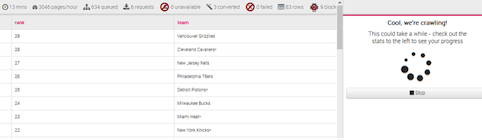
\includegraphics{Fig-3.png}
\caption{Import IO Crawler Output}
\end{figure}

Due to the large number of parameters, a data reduction step must be considered. To further determine the importance of attributes, we decided to construct a decision tree. A decision tree is a flowchart-like tree structure, where each internal node (non-leaf node) denotes a test on an attribute, each branch represents an outcome of the test, and each leaf node (or terminal node) holds a class label. The topmost node in a tree is the root node. Decision tree classification for this project uses information gain as its attribute selection measure. This measure is based on pioneering work by Claude Shannon on information theory, which studied the value or ``information content'' of messages. Let node N represent or hold the tuples of partition D. The attribute with the highest information gain is chosen as the splitting attribute for node N. This attribute minimizes the information needed to classify the tuples in the resulting partitions and reflects the least randomness or ``impurity'' in these partitions. Such an approach minimizes the expected number of tests needed to classify a given tuple and guarantees that a simple (but not necessarily the simplest) tree is found. 

The expected information needed to classify a tuple in D is given by $Info(D) = - \sum_{i=1}^{m} p_{i} log_{2}(p_{i})$ where $p_{i}$ is the probability that an arbitrary tuple in D belongs to class $C_{i}$ and is estimated by $\frac{\textbar C_{i,D} \textbar}{\textbar D\textbar}$. A log function to the base 2 is used, because the information is encoded in bits. Info(D) is just the average amount of information needed to identify the class label of a tuple in D. The information we have is based solely on the proportions of tuples of each class. Info(D) is also known as the entropy of D. Now, suppose we were to partition the tuples in D on some attribute A having v distinct values. If A is discrete-valued, these values correspond directly to the v outcomes of a test on A. Attribute A can be used to split D into v partitions or subsets. These partitions would correspond to the branches grown from node N. Ideally, we would like this partitioning to produce an exact classification of the tuples. That is, we would like for each partition to be pure. However, it is quite likely that the partitions will be impure (e.g., where a partition may contain a collection of tuples from different classes rather than from a single class). How much more information would we still need (after the partitioning) in order to arrive at an exact classification? This amount is measured by $Info_{A}(D) = - \sum_{i=1}^{m} \frac{\textbar D_{j}\textbar}{\textbar D \textbar} \times Info(D_{j})$. The term $\frac{\textbar D_{j}\textbar}{\textbar D \textbar}$ acts as the weight of the $j^{th}$ partition. $Info_{A}(D)$ is the expected information required to classify a tuple from D based on the partitioning by A. The smaller the expected information (still) required, the greater the purity of the partitions. 

Information gain is defined as the difference between the original information requirement (i.e., based on just the proportion of classes) and the new requirement (i.e., obtained after partitioning on A) i.e., $Gain(A) = Info(D) - Info_{A}(D)$ . In other words, Gain(A) tells us how much would be gained by branching on A. It is the expected reduction in the information requirement caused by knowing the value of A. The attribute A with the highest information gain, Gain(A), is chosen as the splitting attribute at node N. This is equivalent to saying that we want to partition on the attribute A that would do the ``best classification'', so that the amount of information still required to finish classifying the tuples is minimal (i.e., minimum $Info_{A}(D)$).     ~\cite{F}

After the appropriate classification is performed, in order to be able to merge these factors together into $I_{perf}$, some normalization must be applied. Because the min-max normalization preserves the relationships among the original data values, it is chosen as the data smoothing technique. Min-max zero-to-one normalization performs a linear transformation on the original data. Suppose that $min_{A}$ and $max_{A}$ are the minimum and maximum values of an attribute, A. Min-max normalization maps a value, v, of A to $v_{0}$ in the range [0:1] by computing $v^{'} = \frac{v - min_{A}}{max_{A}-min{A}}$     ~\cite{G}. Similar procedure could be performed for the individual players. First, players had to be categorized into several categories dependent on their positions such as power forward, small forward, center, shooting guard and point guard. These categories were used to adjust the weights for the parameters factored into the $I_{perf}$. These adjusted parameters could be divided by the salary of the player to determine if a player is overestimated or underestimated. We further could select players with top $I_{perf}$ and combine them into a team trying to maximize $I_{perf}$.


\section{Results and Discussions}
\vspace{0.5em}
\subsection{Team Evaluation}
The first goal of this project is to assess the goodness of a team based on whether it goes to playoff or not. By finding the attributes that represent good teams we can further achieve our primary goal which is evaluating the performance of individual players. To accomplish this task, we need to identify parameters that significantly affect the performance. The datasets we are working with have 26 parameters to choose from, which after data reduction becomes only 9. A decision tree approach is applied to find out the most important attributes form the 9 attributes we choose. When the most important attributes are determined, we merge them into one single factor after applying the min-max normalization to these attributes and use it for describing the performance of a team.

\textbf{Decision Tree: } From the 26 attributes, we reduce the attributes to 9 attributes including FG\%, ORB, DRB, AST, STL, BLK, TOV, PF and PTS/G by ruling out the attributes that are either redundant or relevant. Here the decision is made based on if a team can make to playoff or not. Information gain for all the 9 attributes we choose are calculated to determine the importance of each attribute. We split the past 30 seasons of NBA league into 20 seasons as a training dataset and 10 seasons for model testing which has been shown in Figure 4. To take into account for the temporal changes of the data, we take one season every other two seasons as our testing dataset while the rest of the seasons as the training dataset. In the work presented here, two approaches are used for determining the importance of the attributes. 

\begin{itemize}
\item Within the training dataset, we calculated the information gain for each attribute from the decision tree we construct in Figure 5. By averaging the information gain over these 20 years, the most critical attributes were found. The results are shown in Figure 3. As can be seen from Figure 3, the top five most critical attributes that determine the goodness of a team are FG\%, DRB, TOV, PTS/G, and AST respectively due to their high information gain. The results indicate that to evaluate a player, points which are the most popular and easiest way to evaluate a player is not the best candidate. Instead, the field goal percentage and defense rebound are probably better candidates for player evaluation. 

\begin{figure}[!htb]
\centering
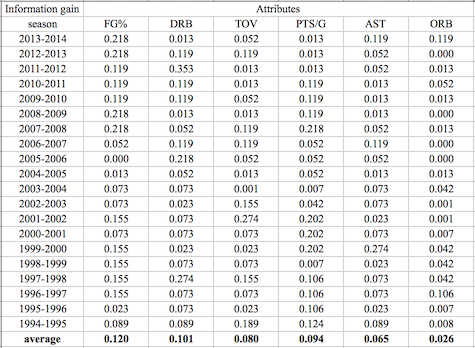
\includegraphics{Fig-24.png}
\caption{The results of information gain in the past 20 seasons}
\end{figure}

\begin{figure}[!htb]
\centering
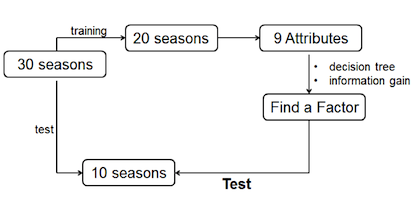
\includegraphics{Fig-5.png}
\caption{Overview of the analytic model}
\end{figure}

\begin{figure}[!htb]
\centering
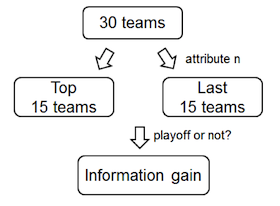
\includegraphics{Fig-6.png}
\caption{1 Layer decision tree for this dataset}
\end{figure}

\item To further validate the five attributes found with approach 1, instead of one layer decision tree, we further split the decision tree into 5 levels and figured out the important attributes as shown in Figure 6. From the results presented in Figure 7, the top five most critical attributes are found to be consistent with approach 1. They are FG\%, DRB, TOV, PTS/G, and AST respectively. Therefore, the following analysis we will focus on these five attributes. 

\begin{figure}[!htb]
\centering
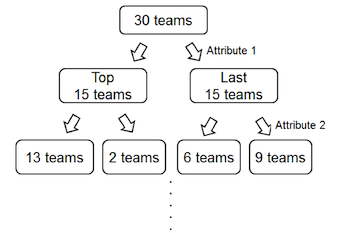
\includegraphics{Fig-7.png}
\caption{Multiple Layers using decision tree for this dataset}
\end{figure}

\begin{figure}[!htb]
\centering
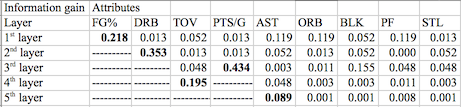
\includegraphics{Fig-25.png}
\caption{The results of information gain for various layers of decision tree}
\end{figure}
\end{itemize}
\textbf{Merge the attributes into a factor $(I_{perf}):$} With the goal of using one single factor to describe a team, we need to merge several most critical attributes. Due to the variations to the scale for different attributes, a min-max normalization approach which is shown in Equation 1 where the subscript N denotes normalized attribute, is applied to unify the scale of various attributes (scale are in 0 $\sim$ 1 after the normalization) and make the merging applicable. An example of normalization is shown in Figure 8 where we normalize the top five most important attributes in the season 2004-2005.

\begin{equation}
Attribute_N = \frac{(Attribute - Min)}{(Max - Min)}
\end{equation}

\begin{figure}[!htb]
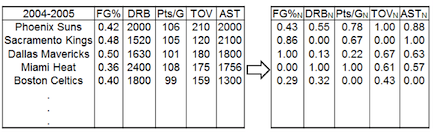
\includegraphics{Fig-8.png}
\caption{An example of min-max normalization}
\end{figure}

After the normalization, we used Equation 2 to merge the important attributes to generate a merged factor which we will name it $I_{perf}$ to describe the performance of a team. However, it should be noted that the sign for the attributes TOV is opposite from the other attributes. This is because TOV contributes negatively to the performance of a team or a player which means the more TOV a team has, the worse performance should be expected. By Equation 2, the new attribute ($I_{perf}$) can be found and it will be used to evaluate the NBA teams in each season. For each season, the 30 NBA teams will be split into the top 15 which have the highest value of $I_{perf}$ and the last 15. In this work, we aim at finding an $I_{perf}$ that can ensure 80\% of the top 15 teams make to the playoff for the testing dataset.

\begin{equation}
I_{perf} = aFG\%_{N} + bDRB_{N} + cTOV_{N} + ...
\end{equation}

To find the $Attribute_{n+1}$, the unknown parameters in Equation 2 are required to be found. Since the scale of the normalized attributes are in 0 $\sim$ 1, we postulate that the unknown parameters are ranging from 0 to 1. For each parameter, a trial and error approach with an interval of 0.1 from 0 to 1 is used for detecting the optimized parameter pair. Here the top three attributes are used for constructing the new factor due to its better accuracy compare to other parameters which can be found in Figure 9. Within the 106 possible combinations of the unknown parameters, the optimized pair is found to be (1.0, 0.6, -0.2) with the training accuracy to be 81.3\% for 20 seasons of the training datasets and the prediction accuracy to be 83.3\% for the test datasets.

\begin{figure}[!htb]
\centering
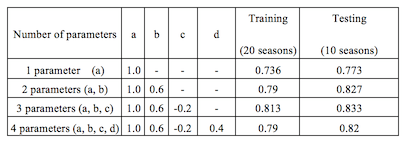
\includegraphics{Fig-9.png}
\caption{The optimized parameters and accuracy for various parameters}
\end{figure}

\subsection{Individual Players}
\vspace{0.5em}
\textbf{Issues and Challenges:} After defining the critical attributes and the important factor ($I_{perf}$) for evaluating teams, we aim at extending these findings to evaluate individual players.  However, several issues should be noticed before applying the factor. First, the attributes such as DRB and TOV for a player are dependent on how many minutes he played for each. The more time a player stays on the court, the more likely for a player to grab rebounds and make turn overs. Normally, the average playing time varies a lot between players. Therefore, instead of looking at the attributes DRB and TOV, DRB/minutes and TOV/minutes are used instead for finding the key factor $I_{perf}$ for players. Second, a basketball team consists of five different positions including center (C), power forward (PF), small forward (SF), shooting guard (SG) and point guard (PG). The FG\% and DRB are generally higher and TOV is normally less for C and PF compare to other positions. Therefore, we need to categorize the players based on the position they played. Otherwise, the analysis would bias against SG and PG. To deal with the issue we split all the players into three categories: 1. Guards (G) including PG and SG, 2. Small forwards (SF) 3. Forwards (F) including C and PF. The categories are shown in Figure 10. The last issue is to normalize the attributes before merging them into one single index. However, if we apply the normalization for all the players together, we would again bias the analysis. Therefore, we apply the min-max normalization for FG\%, DRB/minutes and TOV/minutes in each category instead of whole players before calculating the index for players. 

\begin{figure}[!htb]
\centering
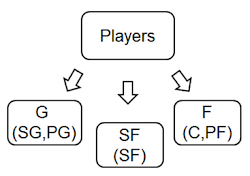
\includegraphics{Fig-10.png}
\caption{Categories of the players}
\end{figure}

\textbf{Merging the Attributes for Individual Players:} Same approach like the last section is used for calculating the index for players. However, for players, how many minutes played is taken into account. Equation 3 where subscript N denotes normalized value is used instead of Equation 2 used in the last section.   

\begin{equation}
I_{perf} = dFG\%_{N} + e \frac{DRB}{minutes_{N}} + f \frac{TOV}{minutes_{N}}
\end{equation}

\vspace{1em}
Via the same approach mentioned in the previous section, we optimized the parameters (d, e, f) for in Equation 3 to find the key factor for players. To verify the accuracy of the description via the factor calculated here, we apply the factor to every player and sum up the factors for every team. By comparing the summation of the factors between teams, we would understand which teams are more likely to perform better and be in the playoff. Theoretically, the higher factor of a team, the better performance and higher probability to be in the playoff should be expected. However, there are two important issues that may bias the comparisons. First, the total number of players in each team varies significantly. The more players a team has, the higher score of the factors would be expected. Thus, the analysis is highly possible to introduce bias to big teams. Second, the number of players in various positions is different across the teams. For example, in the 2014-2015 season, Dallas Mavericks has two centers while Golden State Warriors has three centers. As mentioned above, normally C and PF have higher $I_{perf}$ compared to the other positions. Therefore, the analysis would bias against those teams has less C and PF. To tackle with these issues, we don't investigate all the players of teams. Instead, in each team, the top 3 guards, top 2 small forwards and top 3 power forwards who have the longer ``Minutes Played per Game (MP)'' would be taken into analysis. By doing so, the number of players and the number of players in each position are consistent across all the teams with total 8 players (3 guards, 2 small forwards and 3 power forwards (including centers)). The detailed scheme is shown in Figure 11.

\begin{figure}[!htb]
\centering
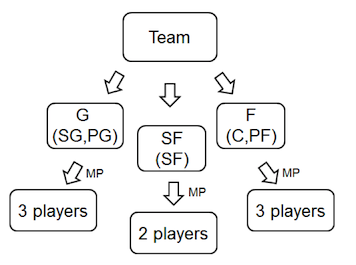
\includegraphics{Fig-11.png}
\caption{The players involved in the analysis}
\end{figure}

Figure 12 lists the summations of the $I_{perf}$ for each team in the West conference and East conference of NBA league in the 2014-2015 season when the $I_{perf}$ is obtained by the parameters (0.6, 0.3, -0.6). From Figure 12, it can be seen that this model can predicts $\frac{5}{8}$ of the teams in the West conference and $\frac{6}{8}$ of the teams in the East conference make to the playoff (In NBA league, the top 8 players in each conference are qualified to be in the playoff.)  This accuracy is 62.5\% for the west conference and 75\% for the east conference which are not perfect but acceptable in terms of its predictive nature. The predictions for individual players have much more issues which are discussed in the above sections compare to team evaluations. On the other hand, there are several important factors we may not be able to predict. 

\begin{itemize}
\item \textbf{The health of players:} Injuries happen a lot in the NBA league and it is unpredictable. Healthy problems sometimes affect the performance of the team a lot especially when key players get injured. For example, Chris Bosh who is an all star power forward in Miami Heat got injured and missed the rest of this season which largely affects the performance of Miami Heat. Miami Heat ended up with $9^{th}$ position in the East conference and didn't make to the playoff.
\item \textbf{Trade of players:} NBA teams trade players in the middle of the season frequently. Sometimes, the deal may involve all star players and affect the ranking of the teams. The effect may be good or bad. For example, in 2014-2015 season, Dallas Mavericks sent several players to Boston and got all star point guard Rajon Rondo. However, this deal didn't bring positive effect to Dallas. Dallas had only 31 wins but 24 loses after the trade which is worse than the 19 wins and 8 loses before the trade. 
\item \textbf{The regression of players:} In the work presented here, we assume that the players would have similar performance as the previous season in order to simplify the model. To predict the regression of players is not a trivial work. There's a literature     ~\cite{H} trying to predict the future performance of several players. However, the result is not good enough to estimate younger players like LeBron James. The regression of players is another possible factor to affect our prediction. 
\end{itemize}

\begin{figure}[!htb]
\centering
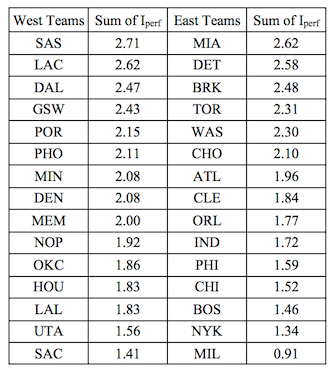
\includegraphics{Fig-12.png}
\caption{The ranking of the NBA teams predicted by $I_{perf}$}
\end{figure}

\subsection{Performance versus Salaries}
\vspace{0.5em}
With the goal of finding undervalued players, salaries must be taken into account. The idea of moneyball is to spend less amount of money but hire valuable players. Therefore, in the work here, we are not targeting those all star players such as Chris Paul, Stephon Curry and Kobe Bryant. We are targeting players who have high enough  $I_{perf}$  but require reasonable salaries. Figures 13-17, the  $I_{perf}$  is plotted against the salaries. It can be noted that the players located in the right down corner are our candidates due to their relatively good performance and low salaries which denotes underestimated players. However, the players on the left up corner are the overestimated players that should be avoided. 

\begin{figure}[!htb]
\centering
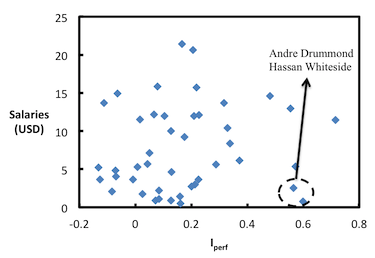
\includegraphics{Fig-14.png}
\caption{Performance plot against player's salaries (Centers)}
\end{figure}

\begin{figure}[!htb]
\centering
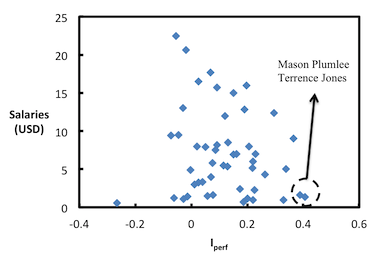
\includegraphics{Fig-15.png}
\caption{Performance plot against player's salaries (Power Forwards)}
\end{figure}

\begin{figure}[!htb]
\centering
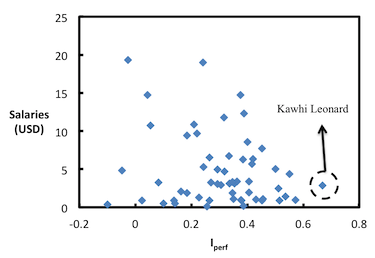
\includegraphics{Fig-16.png}
\caption{Performance plot against player's salaries (Small Forwards)}
\end{figure}

\begin{figure}[!htb]
\centering
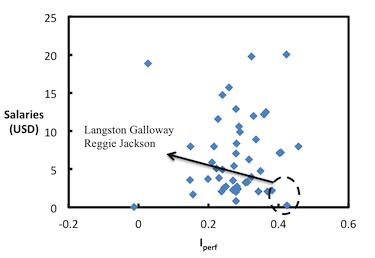
\includegraphics{Fig-17.png}
\caption{Performance plot against player's salaries (Point Guards)}
\end{figure}

\begin{figure}[!htb]
\centering
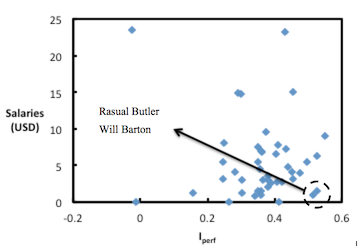
\includegraphics{Fig-18.png}
\caption{Performance plot against player's salaries (Shooting Guard)}
\end{figure}

We have listed down some of the $\frac{I_{perf}}{salaries}$ values in Figures 18-22. which may be a good reference for evaluating NBA players. Depends on the budget and the strategy of a team, different decision may be made based on the information in these figures. Rich team may make decisions based on the value of $I_{perf}$ while small team may put more focus on the value of $\frac{I_{perf}}{salaries}$ to form a more economic and competitive team.

\begin{figure}[!htb]
\centering
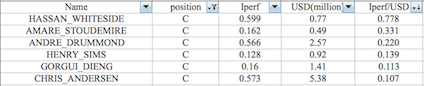
\includegraphics{Fig-19.png}
\caption{The performance and salaries of players (Centers)}
\end{figure}

\begin{figure}[!htb]
\centering
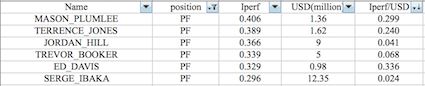
\includegraphics{Fig-20.png}
\caption{The performance and salaries of players (Power Forwards)}
\end{figure}

\begin{figure}[!htb]
\centering
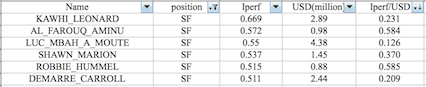
\includegraphics{Fig-21.png}
\caption{The performance and salaries of players (Small Forwards)}
\end{figure}

\begin{figure}[!htb]
\centering
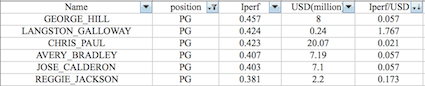
\includegraphics{Fig-22.png}
\caption{The performance and salaries of players (Point Guards)}
\end{figure}

\begin{figure}[!htb]
\centering
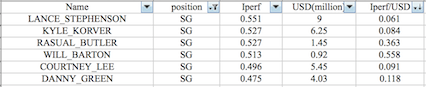
\includegraphics{Fig-23.png}
\caption{The performance and salaries of players (Shooting Guards)}
\end{figure}

\vspace{50em}
\section{Conclusion}
\vspace{0.5em}
To apply the concept of ``Moneyball'' to NBA, we need to figure out what attributes are the most important for describing the performance of a NBA team. Via decision tree approach and information gain calculations, the top five critical attributes are found to be FG\%, DRB, TOV, PTS/G and AST. To achieve the goal of using a single index to predict the performance of a team, a min-max normalization is applied followed by merging the different attributes into one single index ($I_{perf}$). By trial and error, we determine the merging parameters to be (1, 0.6, -0.2). The accuracy of using top three attributes is >80\% for both training datasets and test datasets. When comes to the individual player analysis, several issues including the attribute average varies across different positions and several attributes are time dependent. Therefore, the players are categorized into three groups (G, SF, PF) and normalized within the categories. With the same approach used for team analysis, the best parameters for individual player is (0.6, 0.3, -0.6). By the approach here, we are able to predict the ongoing 2014-2015 season by 2013-2014 player's data. The predict accuracy are $\frac{5}{8}$ for the West conference and $\frac{6}{8}$ for the East conference. The error could come from multiple possibility including the health of the key players, trade in the middle of the seasons and the regression of key players. Finally, we take into account the salaries of the players and find out underestimated players. By doing the scatter plot and the comprehensive table provided in the discussion section, the underestimated and overestimated players are easy to found.

\vspace{2em}
\section{Future Work}
\vspace{0.5em}
We can also apply this model to evaluate the results of old NBA seasons, although it is not as interesting as predicting the on-going or future seasons. However, it is a good way to further justify the approach.

It can be seen that the accuracy of this work is relatively accurate but not perfect. Perhaps, there are other attributes that are important that we didn't take into account. In order to improve the model, we may need to figure out how to describe the attributes that can represent the ``defense'' ability of a player. In NBA statistics, seldom attributes are directly correlated to the defense performance. However, defense always plays a key role in NBA games. We believe if the defense can be taken into account, this model may be significantly improved.
In the present work, the performance of a player is assumed to be similar to the previous season which may not be correct. To improve the model, we may figure out another model to predict the probability of a player. On the other hand, the way we categorize players may not be perfect. In the future we may categorize players in a better and more detailed way. 

\section{Appendix}
\vspace{0.5em}
On my honor, as a University of Colorado at Boulder student, I have neither given nor received unauthorized assistance on this work.

\textbf{Contributions:}

Yu-Ching Kuo: Idea for the course project, Problem Solving, Define Methods to Analyze the results, Slides and Proposal Writing.

Krishna Chaitanya Sripada: Data Cleaning, Coding the project, Analyzing the results, Debugging issues in the code, Proposal and Project Report Writing in LaTeX.

Kirill Novik: Downloaded data, Figured out how to quickly extract data from the Data Source, Proposal Writing and provided suggestions for improvement.

\begin{thebibliography}{}
\vspace{0.5em}
\bibitem{A}Lewis, M. (2003). Moneyball: The art of winning an unfair game. New York: W.W. Norton.
\bibitem{B} Field Goal from Wikipedia \href{http://en.wikipedia.org/wiki/Field_goal}{Field Goal}
\bibitem{C} Sporting Charts. (n.d.). Retrieved April 27, 2015, from \href{http://www.sportingcharts.com/dictionary/nba/effective-field-goal-percentage-efg.aspx}{Effective Field Goal Percentage}
\bibitem{D} Basketball statistics. (n.d.). Retrieved April 27, 2015, from \href{http://en.wikipedia.org/wiki/Basketball_statistics}{Basketball Statistics}
\bibitem{E} Instantly Turn Web Pages into Data. (n.d.). Retrieved April 27, 2015, from \href{https://import.io/}{Import IO}
\bibitem{F} Han, J., \& Kamber, M. (2006). Classification by Decision Tree Induction. In Data mining concepts and techniques (2nd ed., pp. 293-298). Amsterdam: Elsevier.
\bibitem{G} Han, J., \& Kamber, M. (2006). Classification by Decision Tree Induction. In Data integration and transformation (2nd ed., pp. 70-72). Amsterdam: Elsevier.
\setlength{\itemindent}{0.13in}
\bibitem{H} Douglas Hwang. Forecasting NBA Player Performance using a Weibull-Gamma Statistical Timing Model, 2012.
\end{thebibliography}

\end{document}
